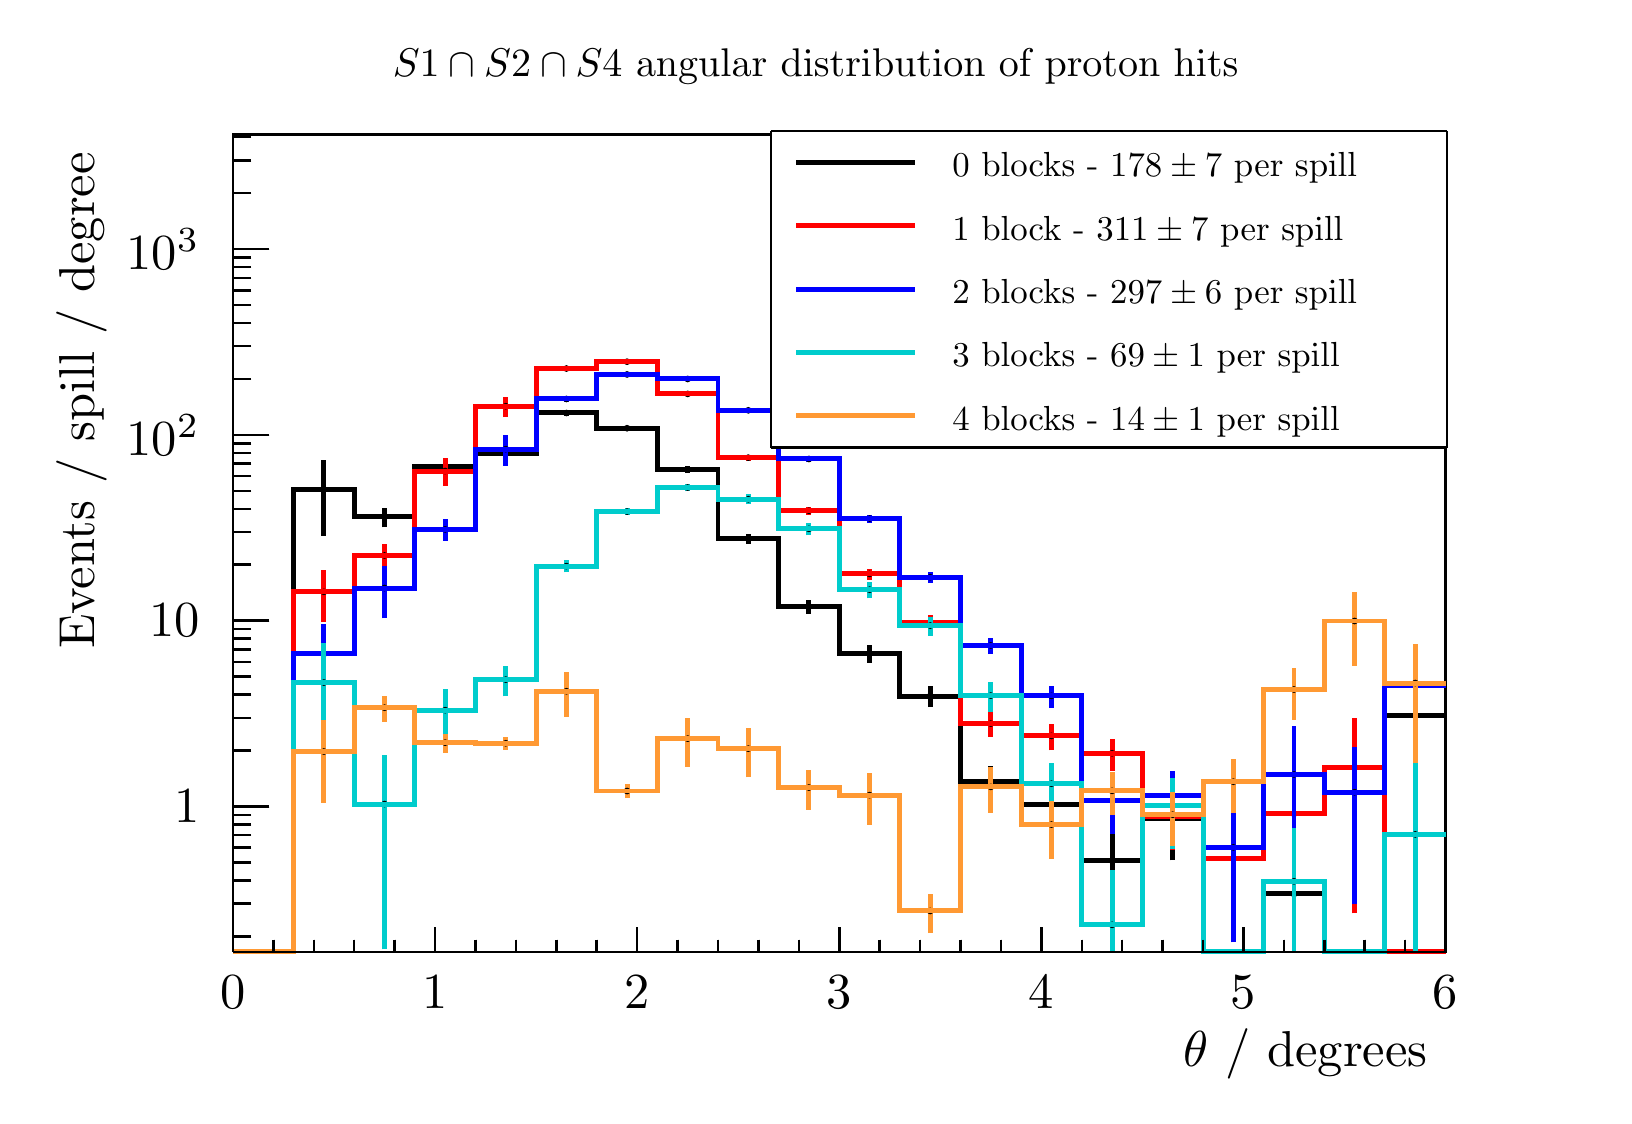
\begin{tikzpicture}
\pgfdeclareplotmark{cross} {
\pgfpathmoveto{\pgfpoint{-0.3\pgfplotmarksize}{\pgfplotmarksize}}
\pgfpathlineto{\pgfpoint{+0.3\pgfplotmarksize}{\pgfplotmarksize}}
\pgfpathlineto{\pgfpoint{+0.3\pgfplotmarksize}{0.3\pgfplotmarksize}}
\pgfpathlineto{\pgfpoint{+1\pgfplotmarksize}{0.3\pgfplotmarksize}}
\pgfpathlineto{\pgfpoint{+1\pgfplotmarksize}{-0.3\pgfplotmarksize}}
\pgfpathlineto{\pgfpoint{+0.3\pgfplotmarksize}{-0.3\pgfplotmarksize}}
\pgfpathlineto{\pgfpoint{+0.3\pgfplotmarksize}{-1.\pgfplotmarksize}}
\pgfpathlineto{\pgfpoint{-0.3\pgfplotmarksize}{-1.\pgfplotmarksize}}
\pgfpathlineto{\pgfpoint{-0.3\pgfplotmarksize}{-0.3\pgfplotmarksize}}
\pgfpathlineto{\pgfpoint{-1.\pgfplotmarksize}{-0.3\pgfplotmarksize}}
\pgfpathlineto{\pgfpoint{-1.\pgfplotmarksize}{0.3\pgfplotmarksize}}
\pgfpathlineto{\pgfpoint{-0.3\pgfplotmarksize}{0.3\pgfplotmarksize}}
\pgfpathclose
\pgfusepathqstroke
}
\pgfdeclareplotmark{cross*} {
\pgfpathmoveto{\pgfpoint{-0.3\pgfplotmarksize}{\pgfplotmarksize}}
\pgfpathlineto{\pgfpoint{+0.3\pgfplotmarksize}{\pgfplotmarksize}}
\pgfpathlineto{\pgfpoint{+0.3\pgfplotmarksize}{0.3\pgfplotmarksize}}
\pgfpathlineto{\pgfpoint{+1\pgfplotmarksize}{0.3\pgfplotmarksize}}
\pgfpathlineto{\pgfpoint{+1\pgfplotmarksize}{-0.3\pgfplotmarksize}}
\pgfpathlineto{\pgfpoint{+0.3\pgfplotmarksize}{-0.3\pgfplotmarksize}}
\pgfpathlineto{\pgfpoint{+0.3\pgfplotmarksize}{-1.\pgfplotmarksize}}
\pgfpathlineto{\pgfpoint{-0.3\pgfplotmarksize}{-1.\pgfplotmarksize}}
\pgfpathlineto{\pgfpoint{-0.3\pgfplotmarksize}{-0.3\pgfplotmarksize}}
\pgfpathlineto{\pgfpoint{-1.\pgfplotmarksize}{-0.3\pgfplotmarksize}}
\pgfpathlineto{\pgfpoint{-1.\pgfplotmarksize}{0.3\pgfplotmarksize}}
\pgfpathlineto{\pgfpoint{-0.3\pgfplotmarksize}{0.3\pgfplotmarksize}}
\pgfpathclose
\pgfusepathqfillstroke
}
\pgfdeclareplotmark{newstar} {
\pgfpathmoveto{\pgfqpoint{0pt}{\pgfplotmarksize}}
\pgfpathlineto{\pgfqpointpolar{44}{0.5\pgfplotmarksize}}
\pgfpathlineto{\pgfqpointpolar{18}{\pgfplotmarksize}}
\pgfpathlineto{\pgfqpointpolar{-20}{0.5\pgfplotmarksize}}
\pgfpathlineto{\pgfqpointpolar{-54}{\pgfplotmarksize}}
\pgfpathlineto{\pgfqpointpolar{-90}{0.5\pgfplotmarksize}}
\pgfpathlineto{\pgfqpointpolar{234}{\pgfplotmarksize}}
\pgfpathlineto{\pgfqpointpolar{198}{0.5\pgfplotmarksize}}
\pgfpathlineto{\pgfqpointpolar{162}{\pgfplotmarksize}}
\pgfpathlineto{\pgfqpointpolar{134}{0.5\pgfplotmarksize}}
\pgfpathclose
\pgfusepathqstroke
}
\pgfdeclareplotmark{newstar*} {
\pgfpathmoveto{\pgfqpoint{0pt}{\pgfplotmarksize}}
\pgfpathlineto{\pgfqpointpolar{44}{0.5\pgfplotmarksize}}
\pgfpathlineto{\pgfqpointpolar{18}{\pgfplotmarksize}}
\pgfpathlineto{\pgfqpointpolar{-20}{0.5\pgfplotmarksize}}
\pgfpathlineto{\pgfqpointpolar{-54}{\pgfplotmarksize}}
\pgfpathlineto{\pgfqpointpolar{-90}{0.5\pgfplotmarksize}}
\pgfpathlineto{\pgfqpointpolar{234}{\pgfplotmarksize}}
\pgfpathlineto{\pgfqpointpolar{198}{0.5\pgfplotmarksize}}
\pgfpathlineto{\pgfqpointpolar{162}{\pgfplotmarksize}}
\pgfpathlineto{\pgfqpointpolar{134}{0.5\pgfplotmarksize}}
\pgfpathclose
\pgfusepathqfillstroke
}
\definecolor{c}{rgb}{1,1,1};
\draw [color=c, fill=c] (0,0) rectangle (20,13.4844);
\draw [color=c, fill=c] (2.6,1.75297) rectangle (18,12.136);
\definecolor{c}{rgb}{0,0,0};
\draw [c,line width=0.9] (2.6,1.75297) -- (2.6,12.136) -- (18,12.136) -- (18,1.75297) -- (2.6,1.75297);
\definecolor{c}{rgb}{1,1,1};
\draw [color=c, fill=c] (2.6,1.75297) rectangle (18,12.136);
\definecolor{c}{rgb}{0,0,0};
\draw [c,line width=0.9] (2.6,1.75297) -- (2.6,12.136) -- (18,12.136) -- (18,1.75297) -- (2.6,1.75297);
\definecolor{c}{rgb}{0,0,0.6};
\draw [c,line width=0.9] (2.6,1.75297) -- (3.37,1.75297) -- (3.37,1.75297) -- (4.14,1.75297) -- (4.14,1.75297) -- (4.91,1.75297) -- (4.91,1.75297) -- (5.68,1.75297) -- (5.68,1.75297) -- (6.45,1.75297) -- (6.45,1.75297) -- (7.22,1.75297) --
 (7.22,1.75297) -- (7.99,1.75297) -- (7.99,1.75297) -- (8.76,1.75297) -- (8.76,1.75297) -- (9.53,1.75297) -- (9.53,1.75297) -- (10.3,1.75297) -- (10.3,1.75297) -- (11.07,1.75297) -- (11.07,1.75297) -- (11.84,1.75297) -- (11.84,1.75297) --
 (12.61,1.75297) -- (12.61,1.75297) -- (13.38,1.75297) -- (13.38,1.75297) -- (14.15,1.75297) -- (14.15,1.75297) -- (14.92,1.75297) -- (14.92,1.75297) -- (15.69,1.75297) -- (15.69,1.75297) -- (16.46,1.75297) -- (16.46,1.75297) -- (17.23,1.75297) --
 (17.23,1.75297) -- (18,1.75297);
\definecolor{c}{rgb}{0,0,0};
\draw [c,line width=0.9] (2.6,1.75297) -- (18,1.75297);
\draw [c,line width=0.9] (2.6,2.06446) -- (2.6,1.75297);
\draw [c,line width=0.9] (3.11333,1.90872) -- (3.11333,1.75297);
\draw [c,line width=0.9] (3.62667,1.90872) -- (3.62667,1.75297);
\draw [c,line width=0.9] (4.14,1.90872) -- (4.14,1.75297);
\draw [c,line width=0.9] (4.65333,1.90872) -- (4.65333,1.75297);
\draw [c,line width=0.9] (5.16667,2.06446) -- (5.16667,1.75297);
\draw [c,line width=0.9] (5.68,1.90872) -- (5.68,1.75297);
\draw [c,line width=0.9] (6.19333,1.90872) -- (6.19333,1.75297);
\draw [c,line width=0.9] (6.70667,1.90872) -- (6.70667,1.75297);
\draw [c,line width=0.9] (7.22,1.90872) -- (7.22,1.75297);
\draw [c,line width=0.9] (7.73333,2.06446) -- (7.73333,1.75297);
\draw [c,line width=0.9] (8.24667,1.90872) -- (8.24667,1.75297);
\draw [c,line width=0.9] (8.76,1.90872) -- (8.76,1.75297);
\draw [c,line width=0.9] (9.27333,1.90872) -- (9.27333,1.75297);
\draw [c,line width=0.9] (9.78667,1.90872) -- (9.78667,1.75297);
\draw [c,line width=0.9] (10.3,2.06446) -- (10.3,1.75297);
\draw [c,line width=0.9] (10.8133,1.90872) -- (10.8133,1.75297);
\draw [c,line width=0.9] (11.3267,1.90872) -- (11.3267,1.75297);
\draw [c,line width=0.9] (11.84,1.90872) -- (11.84,1.75297);
\draw [c,line width=0.9] (12.3533,1.90872) -- (12.3533,1.75297);
\draw [c,line width=0.9] (12.8667,2.06446) -- (12.8667,1.75297);
\draw [c,line width=0.9] (13.38,1.90872) -- (13.38,1.75297);
\draw [c,line width=0.9] (13.8933,1.90872) -- (13.8933,1.75297);
\draw [c,line width=0.9] (14.4067,1.90872) -- (14.4067,1.75297);
\draw [c,line width=0.9] (14.92,1.90872) -- (14.92,1.75297);
\draw [c,line width=0.9] (15.4333,2.06446) -- (15.4333,1.75297);
\draw [c,line width=0.9] (15.9467,1.90872) -- (15.9467,1.75297);
\draw [c,line width=0.9] (16.46,1.90872) -- (16.46,1.75297);
\draw [c,line width=0.9] (16.9733,1.90872) -- (16.9733,1.75297);
\draw [c,line width=0.9] (17.4867,1.90872) -- (17.4867,1.75297);
\draw [c,line width=0.9] (18,2.06446) -- (18,1.75297);
\draw [anchor=base] (2.6,1.0383) node[scale=1.82459, color=c, rotate=0]{0};
\draw [anchor=base] (5.16667,1.0383) node[scale=1.82459, color=c, rotate=0]{1};
\draw [anchor=base] (7.73333,1.0383) node[scale=1.82459, color=c, rotate=0]{2};
\draw [anchor=base] (10.3,1.0383) node[scale=1.82459, color=c, rotate=0]{3};
\draw [anchor=base] (12.8667,1.0383) node[scale=1.82459, color=c, rotate=0]{4};
\draw [anchor=base] (15.4333,1.0383) node[scale=1.82459, color=c, rotate=0]{5};
\draw [anchor=base] (18,1.0383) node[scale=1.82459, color=c, rotate=0]{6};
\draw [anchor= east] (18,0.45847) node[scale=1.82459, color=c, rotate=0]{$\theta$ / degrees};
\draw [c,line width=0.9] (2.6,1.75297) -- (2.6,12.136);
\draw [c,line width=0.9] (2.831,1.95126) -- (2.6,1.95126);
\draw [c,line width=0.9] (2.831,2.36679) -- (2.6,2.36679);
\draw [c,line width=0.9] (2.831,2.66162) -- (2.6,2.66162);
\draw [c,line width=0.9] (2.831,2.8903) -- (2.6,2.8903);
\draw [c,line width=0.9] (2.831,3.07715) -- (2.6,3.07715);
\draw [c,line width=0.9] (2.831,3.23513) -- (2.6,3.23513);
\draw [c,line width=0.9] (2.831,3.37198) -- (2.6,3.37198);
\draw [c,line width=0.9] (2.831,3.49269) -- (2.6,3.49269);
\draw [c,line width=0.9] (3.062,3.60066) -- (2.6,3.60066);
\draw [anchor= east] (2.404,3.60066) node[scale=1.82459, color=c, rotate=0]{1};
\draw [c,line width=0.9] (2.831,4.31103) -- (2.6,4.31103);
\draw [c,line width=0.9] (2.831,4.72656) -- (2.6,4.72656);
\draw [c,line width=0.9] (2.831,5.02139) -- (2.6,5.02139);
\draw [c,line width=0.9] (2.831,5.25007) -- (2.6,5.25007);
\draw [c,line width=0.9] (2.831,5.43692) -- (2.6,5.43692);
\draw [c,line width=0.9] (2.831,5.5949) -- (2.6,5.5949);
\draw [c,line width=0.9] (2.831,5.73175) -- (2.6,5.73175);
\draw [c,line width=0.9] (2.831,5.85245) -- (2.6,5.85245);
\draw [c,line width=0.9] (3.062,5.96043) -- (2.6,5.96043);
\draw [anchor= east] (2.404,5.96043) node[scale=1.82459, color=c, rotate=0]{10};
\draw [c,line width=0.9] (2.831,6.67079) -- (2.6,6.67079);
\draw [c,line width=0.9] (2.831,7.08632) -- (2.6,7.08632);
\draw [c,line width=0.9] (2.831,7.38115) -- (2.6,7.38115);
\draw [c,line width=0.9] (2.831,7.60984) -- (2.6,7.60984);
\draw [c,line width=0.9] (2.831,7.79669) -- (2.6,7.79669);
\draw [c,line width=0.9] (2.831,7.95466) -- (2.6,7.95466);
\draw [c,line width=0.9] (2.831,8.09151) -- (2.6,8.09151);
\draw [c,line width=0.9] (2.831,8.21222) -- (2.6,8.21222);
\draw [c,line width=0.9] (3.062,8.3202) -- (2.6,8.3202);
\draw [anchor= east] (2.404,8.3202) node[scale=1.82459, color=c, rotate=0]{$10^{2}$};
\draw [c,line width=0.9] (2.831,9.03056) -- (2.6,9.03056);
\draw [c,line width=0.9] (2.831,9.44609) -- (2.6,9.44609);
\draw [c,line width=0.9] (2.831,9.74092) -- (2.6,9.74092);
\draw [c,line width=0.9] (2.831,9.9696) -- (2.6,9.9696);
\draw [c,line width=0.9] (2.831,10.1565) -- (2.6,10.1565);
\draw [c,line width=0.9] (2.831,10.3144) -- (2.6,10.3144);
\draw [c,line width=0.9] (2.831,10.4513) -- (2.6,10.4513);
\draw [c,line width=0.9] (2.831,10.572) -- (2.6,10.572);
\draw [c,line width=0.9] (3.062,10.68) -- (2.6,10.68);
\draw [anchor= east] (2.404,10.68) node[scale=1.82459, color=c, rotate=0]{$10^{3}$};
\draw [c,line width=0.9] (2.831,11.3903) -- (2.6,11.3903);
\draw [c,line width=0.9] (2.831,11.8059) -- (2.6,11.8059);
\draw [c,line width=0.9] (2.831,12.1007) -- (2.6,12.1007);
\draw [anchor= east] (0.68,12.136) node[scale=1.82459, color=c, rotate=90]{ Events / spill / degree};
\draw [c,line width=1.8] (3.755,7.03662) -- (3.755,7.62677);
\draw [c,line width=1.8] (3.755,7.62677) -- (3.755,7.99888);
\foreach \P in {(3.755,7.62677)}{\draw[mark options={color=c,fill=c},mark size=2.402402pt,mark=*,mark size=1pt] plot coordinates {\P};}
\draw [c,line width=1.8] (4.525,7.1466) -- (4.525,7.27835);
\draw [c,line width=1.8] (4.525,7.27835) -- (4.525,7.39508);
\foreach \P in {(4.525,7.27835)}{\draw[mark options={color=c,fill=c},mark size=2.402402pt,mark=*,mark size=1pt] plot coordinates {\P};}
\draw [c,line width=1.8] (5.295,7.84132) -- (5.295,7.91274);
\draw [c,line width=1.8] (5.295,7.91274) -- (5.295,7.97951);
\foreach \P in {(5.295,7.91274)}{\draw[mark options={color=c,fill=c},mark size=2.402402pt,mark=*,mark size=1pt] plot coordinates {\P};}
\draw [c,line width=1.8] (6.065,8.04229) -- (6.065,8.08134);
\draw [c,line width=1.8] (6.065,8.08134) -- (6.065,8.11896);
\foreach \P in {(6.065,8.08134)}{\draw[mark options={color=c,fill=c},mark size=2.402402pt,mark=*,mark size=1pt] plot coordinates {\P};}
\draw [c,line width=1.8] (6.835,8.56056) -- (6.835,8.59781);
\draw [c,line width=1.8] (6.835,8.59781) -- (6.835,8.63376);
\foreach \P in {(6.835,8.59781)}{\draw[mark options={color=c,fill=c},mark size=2.402402pt,mark=*,mark size=1pt] plot coordinates {\P};}
\draw [c,line width=1.8] (7.605,8.37354) -- (7.605,8.40444);
\draw [c,line width=1.8] (7.605,8.40444) -- (7.605,8.43445);
\foreach \P in {(7.605,8.40444)}{\draw[mark options={color=c,fill=c},mark size=2.402402pt,mark=*,mark size=1pt] plot coordinates {\P};}
\draw [c,line width=1.8] (8.375,7.84098) -- (8.375,7.88092);
\draw [c,line width=1.8] (8.375,7.88092) -- (8.375,7.91937);
\foreach \P in {(8.375,7.88092)}{\draw[mark options={color=c,fill=c},mark size=2.402402pt,mark=*,mark size=1pt] plot coordinates {\P};}
\draw [c,line width=1.8] (9.145,6.93958) -- (9.145,7.00086);
\draw [c,line width=1.8] (9.145,7.00086) -- (9.145,7.05867);
\foreach \P in {(9.145,7.00086)}{\draw[mark options={color=c,fill=c},mark size=2.402402pt,mark=*,mark size=1pt] plot coordinates {\P};}
\draw [c,line width=1.8] (9.915,6.04796) -- (9.915,6.13934);
\draw [c,line width=1.8] (9.915,6.13934) -- (9.915,6.22323);
\foreach \P in {(9.915,6.13934)}{\draw[mark options={color=c,fill=c},mark size=2.402402pt,mark=*,mark size=1pt] plot coordinates {\P};}
\draw [c,line width=1.8] (10.685,5.42614) -- (10.685,5.54477);
\draw [c,line width=1.8] (10.685,5.54477) -- (10.685,5.65109);
\foreach \P in {(10.685,5.54477)}{\draw[mark options={color=c,fill=c},mark size=2.402402pt,mark=*,mark size=1pt] plot coordinates {\P};}
\draw [c,line width=1.8] (11.455,4.86173) -- (11.455,5.00183);
\draw [c,line width=1.8] (11.455,5.00183) -- (11.455,5.12506);
\foreach \P in {(11.455,5.00183)}{\draw[mark options={color=c,fill=c},mark size=2.402402pt,mark=*,mark size=1pt] plot coordinates {\P};}
\draw [c,line width=1.8] (12.225,3.66036) -- (12.225,3.91178);
\draw [c,line width=1.8] (12.225,3.91178) -- (12.225,4.11351);
\foreach \P in {(12.225,3.91178)}{\draw[mark options={color=c,fill=c},mark size=2.402402pt,mark=*,mark size=1pt] plot coordinates {\P};}
\draw [c,line width=1.8] (12.995,3.32051) -- (12.995,3.62728);
\draw [c,line width=1.8] (12.995,3.62728) -- (12.995,3.86307);
\foreach \P in {(12.995,3.62728)}{\draw[mark options={color=c,fill=c},mark size=2.402402pt,mark=*,mark size=1pt] plot coordinates {\P};}
\draw [c,line width=1.8] (13.765,2.29699) -- (13.765,2.91186);
\draw [c,line width=1.8] (13.765,2.91186) -- (13.765,3.29349);
\foreach \P in {(13.765,2.91186)}{\draw[mark options={color=c,fill=c},mark size=2.402402pt,mark=*,mark size=1pt] plot coordinates {\P};}
\draw [c,line width=1.8] (14.535,2.91498) -- (14.535,3.44952);
\draw [c,line width=1.8] (14.535,3.44952) -- (14.535,3.79904);
\foreach \P in {(14.535,3.44952)}{\draw[mark options={color=c,fill=c},mark size=2.402402pt,mark=*,mark size=1pt] plot coordinates {\P};}
\draw [c,line width=1.8] (16.075,1.75297) -- (16.075,2.48929);
\draw [c,line width=1.8] (16.075,2.48929) -- (16.075,3.04709);
\foreach \P in {(16.075,2.48929)}{\draw[mark options={color=c,fill=c},mark size=2.402402pt,mark=*,mark size=1pt] plot coordinates {\P};}
\draw [c,line width=1.8] (17.615,1.75297) -- (17.615,4.75258);
\draw [c,line width=1.8] (17.615,4.75258) -- (17.615,5.51616);
\foreach \P in {(17.615,4.75258)}{\draw[mark options={color=c,fill=c},mark size=2.402402pt,mark=*,mark size=1pt] plot coordinates {\P};}
\draw [c,line width=1.8] (2.6,1.75297) -- (3.37,1.75297) -- (3.37,7.62677) -- (4.14,7.62677) -- (4.14,7.27835) -- (4.91,7.27835) -- (4.91,7.91274) -- (5.68,7.91274) -- (5.68,8.08134) -- (6.45,8.08134) -- (6.45,8.59781) -- (7.22,8.59781) --
 (7.22,8.40444) -- (7.99,8.40444) -- (7.99,7.88092) -- (8.76,7.88092) -- (8.76,7.00086) -- (9.53,7.00086) -- (9.53,6.13934) -- (10.3,6.13934) -- (10.3,5.54477) -- (11.07,5.54477) -- (11.07,5.00183) -- (11.84,5.00183) -- (11.84,3.91178) --
 (12.61,3.91178) -- (12.61,3.62728) -- (13.38,3.62728) -- (13.38,2.91186) -- (14.15,2.91186) -- (14.15,3.44952) -- (14.92,3.44952) -- (14.92,1.75297) -- (15.69,1.75297) -- (15.69,2.48929) -- (16.46,2.48929) -- (16.46,1.75297) -- (17.23,1.75297) --
 (17.23,4.75258) -- (18,4.75258);
\definecolor{c}{rgb}{1,0,0};
\draw [c,line width=1.8] (3.755,5.93758) -- (3.755,6.32634);
\draw [c,line width=1.8] (3.755,6.32634) -- (3.755,6.60752);
\definecolor{c}{rgb}{0,0,0};
\foreach \P in {(3.755,6.32634)}{\draw[mark options={color=c,fill=c},mark size=2.402402pt,mark=*,mark size=1pt] plot coordinates {\P};}
\definecolor{c}{rgb}{1,0,0};
\draw [c,line width=1.8] (4.525,6.62301) -- (4.525,6.78831);
\draw [c,line width=1.8] (4.525,6.78831) -- (4.525,6.93062);
\definecolor{c}{rgb}{0,0,0};
\foreach \P in {(4.525,6.78831)}{\draw[mark options={color=c,fill=c},mark size=2.402402pt,mark=*,mark size=1pt] plot coordinates {\P};}
\definecolor{c}{rgb}{1,0,0};
\draw [c,line width=1.8] (5.295,7.66978) -- (5.295,7.86087);
\draw [c,line width=1.8] (5.295,7.86087) -- (5.295,8.02187);
\definecolor{c}{rgb}{0,0,0};
\foreach \P in {(5.295,7.86087)}{\draw[mark options={color=c,fill=c},mark size=2.402402pt,mark=*,mark size=1pt] plot coordinates {\P};}
\definecolor{c}{rgb}{1,0,0};
\draw [c,line width=1.8] (6.065,8.54588) -- (6.065,8.68387);
\draw [c,line width=1.8] (6.065,8.68387) -- (6.065,8.80546);
\definecolor{c}{rgb}{0,0,0};
\foreach \P in {(6.065,8.68387)}{\draw[mark options={color=c,fill=c},mark size=2.402402pt,mark=*,mark size=1pt] plot coordinates {\P};}
\definecolor{c}{rgb}{1,0,0};
\draw [c,line width=1.8] (6.835,9.1303) -- (6.835,9.1624);
\draw [c,line width=1.8] (6.835,9.1624) -- (6.835,9.19352);
\definecolor{c}{rgb}{0,0,0};
\foreach \P in {(6.835,9.1624)}{\draw[mark options={color=c,fill=c},mark size=2.402402pt,mark=*,mark size=1pt] plot coordinates {\P};}
\definecolor{c}{rgb}{1,0,0};
\draw [c,line width=1.8] (7.605,9.22788) -- (7.605,9.24923);
\draw [c,line width=1.8] (7.605,9.24923) -- (7.605,9.27015);
\definecolor{c}{rgb}{0,0,0};
\foreach \P in {(7.605,9.24923)}{\draw[mark options={color=c,fill=c},mark size=2.402402pt,mark=*,mark size=1pt] plot coordinates {\P};}
\definecolor{c}{rgb}{1,0,0};
\draw [c,line width=1.8] (8.375,8.81278) -- (8.375,8.84023);
\draw [c,line width=1.8] (8.375,8.84023) -- (8.375,8.86696);
\definecolor{c}{rgb}{0,0,0};
\foreach \P in {(8.375,8.84023)}{\draw[mark options={color=c,fill=c},mark size=2.402402pt,mark=*,mark size=1pt] plot coordinates {\P};}
\definecolor{c}{rgb}{1,0,0};
\draw [c,line width=1.8] (9.145,7.99098) -- (9.145,8.03088);
\draw [c,line width=1.8] (9.145,8.03088) -- (9.145,8.06928);
\definecolor{c}{rgb}{0,0,0};
\foreach \P in {(9.145,8.03088)}{\draw[mark options={color=c,fill=c},mark size=2.402402pt,mark=*,mark size=1pt] plot coordinates {\P};}
\definecolor{c}{rgb}{1,0,0};
\draw [c,line width=1.8] (9.915,7.30528) -- (9.915,7.35634);
\draw [c,line width=1.8] (9.915,7.35634) -- (9.915,7.40498);
\definecolor{c}{rgb}{0,0,0};
\foreach \P in {(9.915,7.35634)}{\draw[mark options={color=c,fill=c},mark size=2.402402pt,mark=*,mark size=1pt] plot coordinates {\P};}
\definecolor{c}{rgb}{1,0,0};
\draw [c,line width=1.8] (10.685,6.48123) -- (10.685,6.55437);
\draw [c,line width=1.8] (10.685,6.55437) -- (10.685,6.62263);
\definecolor{c}{rgb}{0,0,0};
\foreach \P in {(10.685,6.55437)}{\draw[mark options={color=c,fill=c},mark size=2.402402pt,mark=*,mark size=1pt] plot coordinates {\P};}
\definecolor{c}{rgb}{1,0,0};
\draw [c,line width=1.8] (11.455,5.8417) -- (11.455,5.94043);
\draw [c,line width=1.8] (11.455,5.94043) -- (11.455,6.03048);
\definecolor{c}{rgb}{0,0,0};
\foreach \P in {(11.455,5.94043)}{\draw[mark options={color=c,fill=c},mark size=2.402402pt,mark=*,mark size=1pt] plot coordinates {\P};}
\definecolor{c}{rgb}{1,0,0};
\draw [c,line width=1.8] (12.225,4.48443) -- (12.225,4.65313);
\draw [c,line width=1.8] (12.225,4.65313) -- (12.225,4.79794);
\definecolor{c}{rgb}{0,0,0};
\foreach \P in {(12.225,4.65313)}{\draw[mark options={color=c,fill=c},mark size=2.402402pt,mark=*,mark size=1pt] plot coordinates {\P};}
\definecolor{c}{rgb}{1,0,0};
\draw [c,line width=1.8] (12.995,4.31151) -- (12.995,4.49686);
\draw [c,line width=1.8] (12.995,4.49686) -- (12.995,4.65376);
\definecolor{c}{rgb}{0,0,0};
\foreach \P in {(12.995,4.49686)}{\draw[mark options={color=c,fill=c},mark size=2.402402pt,mark=*,mark size=1pt] plot coordinates {\P};}
\definecolor{c}{rgb}{1,0,0};
\draw [c,line width=1.8] (13.765,4.05688) -- (13.765,4.27631);
\draw [c,line width=1.8] (13.765,4.27631) -- (13.765,4.45694);
\definecolor{c}{rgb}{0,0,0};
\foreach \P in {(13.765,4.27631)}{\draw[mark options={color=c,fill=c},mark size=2.402402pt,mark=*,mark size=1pt] plot coordinates {\P};}
\definecolor{c}{rgb}{1,0,0};
\draw [c,line width=1.8] (14.535,3.05022) -- (14.535,3.47547);
\draw [c,line width=1.8] (14.535,3.47547) -- (14.535,3.77512);
\definecolor{c}{rgb}{0,0,0};
\foreach \P in {(14.535,3.47547)}{\draw[mark options={color=c,fill=c},mark size=2.402402pt,mark=*,mark size=1pt] plot coordinates {\P};}
\definecolor{c}{rgb}{1,0,0};
\draw [c,line width=1.8] (15.305,1.96144) -- (15.305,2.94418);
\draw [c,line width=1.8] (15.305,2.94418) -- (15.305,3.43649);
\definecolor{c}{rgb}{0,0,0};
\foreach \P in {(15.305,2.94418)}{\draw[mark options={color=c,fill=c},mark size=2.402402pt,mark=*,mark size=1pt] plot coordinates {\P};}
\definecolor{c}{rgb}{1,0,0};
\draw [c,line width=1.8] (16.075,1.82969) -- (16.075,3.50863);
\draw [c,line width=1.8] (16.075,3.50863) -- (16.075,4.11424);
\definecolor{c}{rgb}{0,0,0};
\foreach \P in {(16.075,3.50863)}{\draw[mark options={color=c,fill=c},mark size=2.402402pt,mark=*,mark size=1pt] plot coordinates {\P};}
\definecolor{c}{rgb}{1,0,0};
\draw [c,line width=1.8] (16.845,2.24331) -- (16.845,4.10113);
\draw [c,line width=1.8] (16.845,4.10113) -- (16.845,4.72426);
\definecolor{c}{rgb}{0,0,0};
\foreach \P in {(16.845,4.10113)}{\draw[mark options={color=c,fill=c},mark size=2.402402pt,mark=*,mark size=1pt] plot coordinates {\P};}
\definecolor{c}{rgb}{1,0,0};
\draw [c,line width=1.8] (2.6,1.75297) -- (3.37,1.75297) -- (3.37,6.32634) -- (4.14,6.32634) -- (4.14,6.78831) -- (4.91,6.78831) -- (4.91,7.86087) -- (5.68,7.86087) -- (5.68,8.68387) -- (6.45,8.68387) -- (6.45,9.1624) -- (7.22,9.1624) --
 (7.22,9.24923) -- (7.99,9.24923) -- (7.99,8.84023) -- (8.76,8.84023) -- (8.76,8.03088) -- (9.53,8.03088) -- (9.53,7.35634) -- (10.3,7.35634) -- (10.3,6.55437) -- (11.07,6.55437) -- (11.07,5.94043) -- (11.84,5.94043) -- (11.84,4.65313) --
 (12.61,4.65313) -- (12.61,4.49686) -- (13.38,4.49686) -- (13.38,4.27631) -- (14.15,4.27631) -- (14.15,3.47547) -- (14.92,3.47547) -- (14.92,2.94418) -- (15.69,2.94418) -- (15.69,3.50863) -- (16.46,3.50863) -- (16.46,4.10113) -- (17.23,4.10113) --
 (17.23,1.75297) -- (18,1.75297);
\definecolor{c}{rgb}{0,0,1};
\draw [c,line width=1.8] (3.755,4.92948) -- (3.755,5.53967);
\draw [c,line width=1.8] (3.755,5.53967) -- (3.755,5.91951);
\definecolor{c}{rgb}{0,0,0};
\foreach \P in {(3.755,5.53967)}{\draw[mark options={color=c,fill=c},mark size=2.402402pt,mark=*,mark size=1pt] plot coordinates {\P};}
\definecolor{c}{rgb}{0,0,1};
\draw [c,line width=1.8] (4.525,5.98896) -- (4.525,6.37504);
\draw [c,line width=1.8] (4.525,6.37504) -- (4.525,6.65481);
\definecolor{c}{rgb}{0,0,0};
\foreach \P in {(4.525,6.37504)}{\draw[mark options={color=c,fill=c},mark size=2.402402pt,mark=*,mark size=1pt] plot coordinates {\P};}
\definecolor{c}{rgb}{0,0,1};
\draw [c,line width=1.8] (5.295,6.97604) -- (5.295,7.11947);
\draw [c,line width=1.8] (5.295,7.11947) -- (5.295,7.24527);
\definecolor{c}{rgb}{0,0,0};
\foreach \P in {(5.295,7.11947)}{\draw[mark options={color=c,fill=c},mark size=2.402402pt,mark=*,mark size=1pt] plot coordinates {\P};}
\definecolor{c}{rgb}{0,0,1};
\draw [c,line width=1.8] (6.065,7.92853) -- (6.065,8.13869);
\draw [c,line width=1.8] (6.065,8.13869) -- (6.065,8.313);
\definecolor{c}{rgb}{0,0,0};
\foreach \P in {(6.065,8.13869)}{\draw[mark options={color=c,fill=c},mark size=2.402402pt,mark=*,mark size=1pt] plot coordinates {\P};}
\definecolor{c}{rgb}{0,0,1};
\draw [c,line width=1.8] (6.835,8.74058) -- (6.835,8.77582);
\draw [c,line width=1.8] (6.835,8.77582) -- (6.835,8.80988);
\definecolor{c}{rgb}{0,0,0};
\foreach \P in {(6.835,8.77582)}{\draw[mark options={color=c,fill=c},mark size=2.402402pt,mark=*,mark size=1pt] plot coordinates {\P};}
\definecolor{c}{rgb}{0,0,1};
\draw [c,line width=1.8] (7.605,9.06713) -- (7.605,9.08725);
\draw [c,line width=1.8] (7.605,9.08725) -- (7.605,9.10698);
\definecolor{c}{rgb}{0,0,0};
\foreach \P in {(7.605,9.08725)}{\draw[mark options={color=c,fill=c},mark size=2.402402pt,mark=*,mark size=1pt] plot coordinates {\P};}
\definecolor{c}{rgb}{0,0,1};
\draw [c,line width=1.8] (8.375,9.00595) -- (8.375,9.02976);
\draw [c,line width=1.8] (8.375,9.02976) -- (8.375,9.05303);
\definecolor{c}{rgb}{0,0,0};
\foreach \P in {(8.375,9.02976)}{\draw[mark options={color=c,fill=c},mark size=2.402402pt,mark=*,mark size=1pt] plot coordinates {\P};}
\definecolor{c}{rgb}{0,0,1};
\draw [c,line width=1.8] (9.145,8.6011) -- (9.145,8.63177);
\draw [c,line width=1.8] (9.145,8.63177) -- (9.145,8.66154);
\definecolor{c}{rgb}{0,0,0};
\foreach \P in {(9.145,8.63177)}{\draw[mark options={color=c,fill=c},mark size=2.402402pt,mark=*,mark size=1pt] plot coordinates {\P};}
\definecolor{c}{rgb}{0,0,1};
\draw [c,line width=1.8] (9.915,7.97383) -- (9.915,8.01383);
\draw [c,line width=1.8] (9.915,8.01383) -- (9.915,8.05232);
\definecolor{c}{rgb}{0,0,0};
\foreach \P in {(9.915,8.01383)}{\draw[mark options={color=c,fill=c},mark size=2.402402pt,mark=*,mark size=1pt] plot coordinates {\P};}
\definecolor{c}{rgb}{0,0,1};
\draw [c,line width=1.8] (10.685,7.20292) -- (10.685,7.25699);
\draw [c,line width=1.8] (10.685,7.25699) -- (10.685,7.30836);
\definecolor{c}{rgb}{0,0,0};
\foreach \P in {(10.685,7.25699)}{\draw[mark options={color=c,fill=c},mark size=2.402402pt,mark=*,mark size=1pt] plot coordinates {\P};}
\definecolor{c}{rgb}{0,0,1};
\draw [c,line width=1.8] (11.455,6.43814) -- (11.455,6.51221);
\draw [c,line width=1.8] (11.455,6.51221) -- (11.455,6.58128);
\definecolor{c}{rgb}{0,0,0};
\foreach \P in {(11.455,6.51221)}{\draw[mark options={color=c,fill=c},mark size=2.402402pt,mark=*,mark size=1pt] plot coordinates {\P};}
\definecolor{c}{rgb}{0,0,1};
\draw [c,line width=1.8] (12.225,5.53506) -- (12.225,5.64553);
\draw [c,line width=1.8] (12.225,5.64553) -- (12.225,5.74525);
\definecolor{c}{rgb}{0,0,0};
\foreach \P in {(12.225,5.64553)}{\draw[mark options={color=c,fill=c},mark size=2.402402pt,mark=*,mark size=1pt] plot coordinates {\P};}
\definecolor{c}{rgb}{0,0,1};
\draw [c,line width=1.8] (12.995,4.85753) -- (12.995,5.00496);
\draw [c,line width=1.8] (12.995,5.00496) -- (12.995,5.13381);
\definecolor{c}{rgb}{0,0,0};
\foreach \P in {(12.995,5.00496)}{\draw[mark options={color=c,fill=c},mark size=2.402402pt,mark=*,mark size=1pt] plot coordinates {\P};}
\definecolor{c}{rgb}{0,0,1};
\draw [c,line width=1.8] (13.765,3.25013) -- (13.765,3.67643);
\draw [c,line width=1.8] (13.765,3.67643) -- (13.765,3.9766);
\definecolor{c}{rgb}{0,0,0};
\foreach \P in {(13.765,3.67643)}{\draw[mark options={color=c,fill=c},mark size=2.402402pt,mark=*,mark size=1pt] plot coordinates {\P};}
\definecolor{c}{rgb}{0,0,1};
\draw [c,line width=1.8] (14.535,3.28304) -- (14.535,3.73631);
\draw [c,line width=1.8] (14.535,3.73631) -- (14.535,4.04949);
\definecolor{c}{rgb}{0,0,0};
\foreach \P in {(14.535,3.73631)}{\draw[mark options={color=c,fill=c},mark size=2.402402pt,mark=*,mark size=1pt] plot coordinates {\P};}
\definecolor{c}{rgb}{0,0,1};
\draw [c,line width=1.8] (15.305,1.87596) -- (15.305,3.08101);
\draw [c,line width=1.8] (15.305,3.08101) -- (15.305,3.61965);
\definecolor{c}{rgb}{0,0,0};
\foreach \P in {(15.305,3.08101)}{\draw[mark options={color=c,fill=c},mark size=2.402402pt,mark=*,mark size=1pt] plot coordinates {\P};}
\definecolor{c}{rgb}{0,0,1};
\draw [c,line width=1.8] (16.075,2.16853) -- (16.075,4.00697);
\draw [c,line width=1.8] (16.075,4.00697) -- (16.075,4.62836);
\definecolor{c}{rgb}{0,0,0};
\foreach \P in {(16.075,4.00697)}{\draw[mark options={color=c,fill=c},mark size=2.402402pt,mark=*,mark size=1pt] plot coordinates {\P};}
\definecolor{c}{rgb}{0,0,1};
\draw [c,line width=1.8] (16.845,2.35724) -- (16.845,3.78143);
\draw [c,line width=1.8] (16.845,3.78143) -- (16.845,4.35543);
\definecolor{c}{rgb}{0,0,0};
\foreach \P in {(16.845,3.78143)}{\draw[mark options={color=c,fill=c},mark size=2.402402pt,mark=*,mark size=1pt] plot coordinates {\P};}
\definecolor{c}{rgb}{0,0,1};
\draw [c,line width=1.8] (17.615,4.13319) -- (17.615,5.13955);
\draw [c,line width=1.8] (17.615,5.13955) -- (17.615,5.63739);
\definecolor{c}{rgb}{0,0,0};
\foreach \P in {(17.615,5.13955)}{\draw[mark options={color=c,fill=c},mark size=2.402402pt,mark=*,mark size=1pt] plot coordinates {\P};}
\definecolor{c}{rgb}{0,0,1};
\draw [c,line width=1.8] (2.6,1.75297) -- (3.37,1.75297) -- (3.37,5.53967) -- (4.14,5.53967) -- (4.14,6.37504) -- (4.91,6.37504) -- (4.91,7.11947) -- (5.68,7.11947) -- (5.68,8.13869) -- (6.45,8.13869) -- (6.45,8.77582) -- (7.22,8.77582) --
 (7.22,9.08725) -- (7.99,9.08725) -- (7.99,9.02976) -- (8.76,9.02976) -- (8.76,8.63177) -- (9.53,8.63177) -- (9.53,8.01383) -- (10.3,8.01383) -- (10.3,7.25699) -- (11.07,7.25699) -- (11.07,6.51221) -- (11.84,6.51221) -- (11.84,5.64553) --
 (12.61,5.64553) -- (12.61,5.00496) -- (13.38,5.00496) -- (13.38,3.67643) -- (14.15,3.67643) -- (14.15,3.73631) -- (14.92,3.73631) -- (14.92,3.08101) -- (15.69,3.08101) -- (15.69,4.00697) -- (16.46,4.00697) -- (16.46,3.78143) -- (17.23,3.78143) --
 (17.23,5.13955) -- (18,5.13955);
\definecolor{c}{rgb}{0,0.8,0.8};
\draw [c,line width=1.8] (3.755,4.17313) -- (3.755,5.17438);
\draw [c,line width=1.8] (3.755,5.17438) -- (3.755,5.67103);
\definecolor{c}{rgb}{0,0,0};
\foreach \P in {(3.755,5.17438)}{\draw[mark options={color=c,fill=c},mark size=2.402402pt,mark=*,mark size=1pt] plot coordinates {\P};}
\definecolor{c}{rgb}{0,0.8,0.8};
\draw [c,line width=1.8] (4.525,1.7854) -- (4.525,3.63132);
\draw [c,line width=1.8] (4.525,3.63132) -- (4.525,4.25338);
\definecolor{c}{rgb}{0,0,0};
\foreach \P in {(4.525,3.63132)}{\draw[mark options={color=c,fill=c},mark size=2.402402pt,mark=*,mark size=1pt] plot coordinates {\P};}
\definecolor{c}{rgb}{0,0.8,0.8};
\draw [c,line width=1.8] (5.295,4.44841) -- (5.295,4.82399);
\draw [c,line width=1.8] (5.295,4.82399) -- (5.295,5.09824);
\definecolor{c}{rgb}{0,0,0};
\foreach \P in {(5.295,4.82399)}{\draw[mark options={color=c,fill=c},mark size=2.402402pt,mark=*,mark size=1pt] plot coordinates {\P};}
\definecolor{c}{rgb}{0,0.8,0.8};
\draw [c,line width=1.8] (6.065,4.99757) -- (6.065,5.21162);
\draw [c,line width=1.8] (6.065,5.21162) -- (6.065,5.3886);
\definecolor{c}{rgb}{0,0,0};
\foreach \P in {(6.065,5.21162)}{\draw[mark options={color=c,fill=c},mark size=2.402402pt,mark=*,mark size=1pt] plot coordinates {\P};}
\definecolor{c}{rgb}{0,0.8,0.8};
\draw [c,line width=1.8] (6.835,6.57423) -- (6.835,6.65308);
\draw [c,line width=1.8] (6.835,6.65308) -- (6.835,6.72629);
\definecolor{c}{rgb}{0,0,0};
\foreach \P in {(6.835,6.65308)}{\draw[mark options={color=c,fill=c},mark size=2.402402pt,mark=*,mark size=1pt] plot coordinates {\P};}
\definecolor{c}{rgb}{0,0.8,0.8};
\draw [c,line width=1.8] (7.605,7.30133) -- (7.605,7.34573);
\draw [c,line width=1.8] (7.605,7.34573) -- (7.605,7.38828);
\definecolor{c}{rgb}{0,0,0};
\foreach \P in {(7.605,7.34573)}{\draw[mark options={color=c,fill=c},mark size=2.402402pt,mark=*,mark size=1pt] plot coordinates {\P};}
\definecolor{c}{rgb}{0,0.8,0.8};
\draw [c,line width=1.8] (8.375,7.60217) -- (8.375,7.65084);
\draw [c,line width=1.8] (8.375,7.65084) -- (8.375,7.69729);
\definecolor{c}{rgb}{0,0,0};
\foreach \P in {(8.375,7.65084)}{\draw[mark options={color=c,fill=c},mark size=2.402402pt,mark=*,mark size=1pt] plot coordinates {\P};}
\definecolor{c}{rgb}{0,0.8,0.8};
\draw [c,line width=1.8] (9.145,7.43568) -- (9.145,7.50217);
\draw [c,line width=1.8] (9.145,7.50217) -- (9.145,7.56461);
\definecolor{c}{rgb}{0,0,0};
\foreach \P in {(9.145,7.50217)}{\draw[mark options={color=c,fill=c},mark size=2.402402pt,mark=*,mark size=1pt] plot coordinates {\P};}
\definecolor{c}{rgb}{0,0.8,0.8};
\draw [c,line width=1.8] (9.915,7.04267) -- (9.915,7.12627);
\draw [c,line width=1.8] (9.915,7.12627) -- (9.915,7.20356);
\definecolor{c}{rgb}{0,0,0};
\foreach \P in {(9.915,7.12627)}{\draw[mark options={color=c,fill=c},mark size=2.402402pt,mark=*,mark size=1pt] plot coordinates {\P};}
\definecolor{c}{rgb}{0,0.8,0.8};
\draw [c,line width=1.8] (10.685,6.24395) -- (10.685,6.35391);
\draw [c,line width=1.8] (10.685,6.35391) -- (10.685,6.45322);
\definecolor{c}{rgb}{0,0,0};
\foreach \P in {(10.685,6.35391)}{\draw[mark options={color=c,fill=c},mark size=2.402402pt,mark=*,mark size=1pt] plot coordinates {\P};}
\definecolor{c}{rgb}{0,0.8,0.8};
\draw [c,line width=1.8] (11.455,5.77127) -- (11.455,5.89854);
\draw [c,line width=1.8] (11.455,5.89854) -- (11.455,6.01175);
\definecolor{c}{rgb}{0,0,0};
\foreach \P in {(11.455,5.89854)}{\draw[mark options={color=c,fill=c},mark size=2.402402pt,mark=*,mark size=1pt] plot coordinates {\P};}
\definecolor{c}{rgb}{0,0.8,0.8};
\draw [c,line width=1.8] (12.225,4.80242) -- (12.225,5.00888);
\draw [c,line width=1.8] (12.225,5.00888) -- (12.225,5.18064);
\definecolor{c}{rgb}{0,0,0};
\foreach \P in {(12.225,5.00888)}{\draw[mark options={color=c,fill=c},mark size=2.402402pt,mark=*,mark size=1pt] plot coordinates {\P};}
\definecolor{c}{rgb}{0,0.8,0.8};
\draw [c,line width=1.8] (12.995,3.52802) -- (12.995,3.88988);
\draw [c,line width=1.8] (12.995,3.88988) -- (12.995,4.15678);
\definecolor{c}{rgb}{0,0,0};
\foreach \P in {(12.995,3.88988)}{\draw[mark options={color=c,fill=c},mark size=2.402402pt,mark=*,mark size=1pt] plot coordinates {\P};}
\definecolor{c}{rgb}{0,0.8,0.8};
\draw [c,line width=1.8] (13.765,1.75297) -- (13.765,2.09732);
\draw [c,line width=1.8] (13.765,2.09732) -- (13.765,2.79492);
\definecolor{c}{rgb}{0,0,0};
\foreach \P in {(13.765,2.09732)}{\draw[mark options={color=c,fill=c},mark size=2.402402pt,mark=*,mark size=1pt] plot coordinates {\P};}
\definecolor{c}{rgb}{0,0.8,0.8};
\draw [c,line width=1.8] (14.535,3.06499) -- (14.535,3.61);
\draw [c,line width=1.8] (14.535,3.61) -- (14.535,3.96391);
\definecolor{c}{rgb}{0,0,0};
\foreach \P in {(14.535,3.61)}{\draw[mark options={color=c,fill=c},mark size=2.402402pt,mark=*,mark size=1pt] plot coordinates {\P};}
\definecolor{c}{rgb}{0,0.8,0.8};
\draw [c,line width=1.8] (16.075,1.75297) -- (16.075,2.64999);
\draw [c,line width=1.8] (16.075,2.64999) -- (16.075,3.33125);
\definecolor{c}{rgb}{0,0,0};
\foreach \P in {(16.075,2.64999)}{\draw[mark options={color=c,fill=c},mark size=2.402402pt,mark=*,mark size=1pt] plot coordinates {\P};}
\definecolor{c}{rgb}{0,0.8,0.8};
\draw [c,line width=1.8] (17.615,1.75297) -- (17.615,3.24602);
\draw [c,line width=1.8] (17.615,3.24602) -- (17.615,4.29827);
\definecolor{c}{rgb}{0,0,0};
\foreach \P in {(17.615,3.24602)}{\draw[mark options={color=c,fill=c},mark size=2.402402pt,mark=*,mark size=1pt] plot coordinates {\P};}
\definecolor{c}{rgb}{0,0.8,0.8};
\draw [c,line width=1.8] (2.6,1.75297) -- (3.37,1.75297) -- (3.37,5.17438) -- (4.14,5.17438) -- (4.14,3.63132) -- (4.91,3.63132) -- (4.91,4.82399) -- (5.68,4.82399) -- (5.68,5.21162) -- (6.45,5.21162) -- (6.45,6.65308) -- (7.22,6.65308) --
 (7.22,7.34573) -- (7.99,7.34573) -- (7.99,7.65084) -- (8.76,7.65084) -- (8.76,7.50217) -- (9.53,7.50217) -- (9.53,7.12627) -- (10.3,7.12627) -- (10.3,6.35391) -- (11.07,6.35391) -- (11.07,5.89854) -- (11.84,5.89854) -- (11.84,5.00888) --
 (12.61,5.00888) -- (12.61,3.88988) -- (13.38,3.88988) -- (13.38,2.09732) -- (14.15,2.09732) -- (14.15,3.61) -- (14.92,3.61) -- (14.92,1.75297) -- (15.69,1.75297) -- (15.69,2.64999) -- (16.46,2.64999) -- (16.46,1.75297) -- (17.23,1.75297) --
 (17.23,3.24602) -- (18,3.24602);
\definecolor{c}{rgb}{1,0.6,0.2};
\draw [c,line width=1.8] (3.755,3.64682) -- (3.755,4.29819);
\draw [c,line width=1.8] (3.755,4.29819) -- (3.755,4.69328);
\definecolor{c}{rgb}{0,0,0};
\foreach \P in {(3.755,4.29819)}{\draw[mark options={color=c,fill=c},mark size=2.402402pt,mark=*,mark size=1pt] plot coordinates {\P};}
\definecolor{c}{rgb}{1,0.6,0.2};
\draw [c,line width=1.8] (4.525,4.67827) -- (4.525,4.85504);
\draw [c,line width=1.8] (4.525,4.85504) -- (4.525,5.00576);
\definecolor{c}{rgb}{0,0,0};
\foreach \P in {(4.525,4.85504)}{\draw[mark options={color=c,fill=c},mark size=2.402402pt,mark=*,mark size=1pt] plot coordinates {\P};}
\definecolor{c}{rgb}{1,0.6,0.2};
\draw [c,line width=1.8] (5.295,4.28453) -- (5.295,4.411);
\draw [c,line width=1.8] (5.295,4.411) -- (5.295,4.52357);
\definecolor{c}{rgb}{0,0,0};
\foreach \P in {(5.295,4.411)}{\draw[mark options={color=c,fill=c},mark size=2.402402pt,mark=*,mark size=1pt] plot coordinates {\P};}
\definecolor{c}{rgb}{1,0.6,0.2};
\draw [c,line width=1.8] (6.065,4.32267) -- (6.065,4.40343);
\draw [c,line width=1.8] (6.065,4.40343) -- (6.065,4.47828);
\definecolor{c}{rgb}{0,0,0};
\foreach \P in {(6.065,4.40343)}{\draw[mark options={color=c,fill=c},mark size=2.402402pt,mark=*,mark size=1pt] plot coordinates {\P};}
\definecolor{c}{rgb}{1,0.6,0.2};
\draw [c,line width=1.8] (6.835,4.74071) -- (6.835,5.06405);
\draw [c,line width=1.8] (6.835,5.06405) -- (6.835,5.30947);
\definecolor{c}{rgb}{0,0,0};
\foreach \P in {(6.835,5.06405)}{\draw[mark options={color=c,fill=c},mark size=2.402402pt,mark=*,mark size=1pt] plot coordinates {\P};}
\definecolor{c}{rgb}{1,0.6,0.2};
\draw [c,line width=1.8] (7.605,3.70709) -- (7.605,3.79725);
\draw [c,line width=1.8] (7.605,3.79725) -- (7.605,3.88012);
\definecolor{c}{rgb}{0,0,0};
\foreach \P in {(7.605,3.79725)}{\draw[mark options={color=c,fill=c},mark size=2.402402pt,mark=*,mark size=1pt] plot coordinates {\P};}
\definecolor{c}{rgb}{1,0.6,0.2};
\draw [c,line width=1.8] (8.375,4.10239) -- (8.375,4.46227);
\draw [c,line width=1.8] (8.375,4.46227) -- (8.375,4.72809);
\definecolor{c}{rgb}{0,0,0};
\foreach \P in {(8.375,4.46227)}{\draw[mark options={color=c,fill=c},mark size=2.402402pt,mark=*,mark size=1pt] plot coordinates {\P};}
\definecolor{c}{rgb}{1,0.6,0.2};
\draw [c,line width=1.8] (9.145,3.97036) -- (9.145,4.33499);
\draw [c,line width=1.8] (9.145,4.33499) -- (9.145,4.60338);
\definecolor{c}{rgb}{0,0,0};
\foreach \P in {(9.145,4.33499)}{\draw[mark options={color=c,fill=c},mark size=2.402402pt,mark=*,mark size=1pt] plot coordinates {\P};}
\definecolor{c}{rgb}{1,0.6,0.2};
\draw [c,line width=1.8] (9.915,3.55808) -- (9.915,3.84073);
\draw [c,line width=1.8] (9.915,3.84073) -- (9.915,4.06203);
\definecolor{c}{rgb}{0,0,0};
\foreach \P in {(9.915,3.84073)}{\draw[mark options={color=c,fill=c},mark size=2.402402pt,mark=*,mark size=1pt] plot coordinates {\P};}
\definecolor{c}{rgb}{1,0.6,0.2};
\draw [c,line width=1.8] (10.685,3.36741) -- (10.685,3.74462);
\draw [c,line width=1.8] (10.685,3.74462) -- (10.685,4.01974);
\definecolor{c}{rgb}{0,0,0};
\foreach \P in {(10.685,3.74462)}{\draw[mark options={color=c,fill=c},mark size=2.402402pt,mark=*,mark size=1pt] plot coordinates {\P};}
\definecolor{c}{rgb}{1,0.6,0.2};
\draw [c,line width=1.8] (11.455,1.99296) -- (11.455,2.27381);
\draw [c,line width=1.8] (11.455,2.27381) -- (11.455,2.49402);
\definecolor{c}{rgb}{0,0,0};
\foreach \P in {(11.455,2.27381)}{\draw[mark options={color=c,fill=c},mark size=2.402402pt,mark=*,mark size=1pt] plot coordinates {\P};}
\definecolor{c}{rgb}{1,0.6,0.2};
\draw [c,line width=1.8] (12.225,3.51777) -- (12.225,3.84946);
\draw [c,line width=1.8] (12.225,3.84946) -- (12.225,4.09965);
\definecolor{c}{rgb}{0,0,0};
\foreach \P in {(12.225,3.84946)}{\draw[mark options={color=c,fill=c},mark size=2.402402pt,mark=*,mark size=1pt] plot coordinates {\P};}
\definecolor{c}{rgb}{1,0.6,0.2};
\draw [c,line width=1.8] (12.995,2.93764) -- (12.995,3.37048);
\draw [c,line width=1.8] (12.995,3.37048) -- (12.995,3.67385);
\definecolor{c}{rgb}{0,0,0};
\foreach \P in {(12.995,3.37048)}{\draw[mark options={color=c,fill=c},mark size=2.402402pt,mark=*,mark size=1pt] plot coordinates {\P};}
\definecolor{c}{rgb}{1,0.6,0.2};
\draw [c,line width=1.8] (13.765,3.49163) -- (13.765,3.79909);
\draw [c,line width=1.8] (13.765,3.79909) -- (13.765,4.03528);
\definecolor{c}{rgb}{0,0,0};
\foreach \P in {(13.765,3.79909)}{\draw[mark options={color=c,fill=c},mark size=2.402402pt,mark=*,mark size=1pt] plot coordinates {\P};}
\definecolor{c}{rgb}{1,0.6,0.2};
\draw [c,line width=1.8] (14.535,3.10383) -- (14.535,3.49593);
\draw [c,line width=1.8] (14.535,3.49593) -- (14.535,3.77884);
\definecolor{c}{rgb}{0,0,0};
\foreach \P in {(14.535,3.49593)}{\draw[mark options={color=c,fill=c},mark size=2.402402pt,mark=*,mark size=1pt] plot coordinates {\P};}
\definecolor{c}{rgb}{1,0.6,0.2};
\draw [c,line width=1.8] (15.305,3.52371) -- (15.305,3.91517);
\draw [c,line width=1.8] (15.305,3.91517) -- (15.305,4.19775);
\definecolor{c}{rgb}{0,0,0};
\foreach \P in {(15.305,3.91517)}{\draw[mark options={color=c,fill=c},mark size=2.402402pt,mark=*,mark size=1pt] plot coordinates {\P};}
\definecolor{c}{rgb}{1,0.6,0.2};
\draw [c,line width=1.8] (16.075,4.7038) -- (16.075,5.08605);
\draw [c,line width=1.8] (16.075,5.08605) -- (16.075,5.36382);
\definecolor{c}{rgb}{0,0,0};
\foreach \P in {(16.075,5.08605)}{\draw[mark options={color=c,fill=c},mark size=2.402402pt,mark=*,mark size=1pt] plot coordinates {\P};}
\definecolor{c}{rgb}{1,0.6,0.2};
\draw [c,line width=1.8] (16.845,5.38628) -- (16.845,5.9562);
\draw [c,line width=1.8] (16.845,5.9562) -- (16.845,6.32028);
\definecolor{c}{rgb}{0,0,0};
\foreach \P in {(16.845,5.9562)}{\draw[mark options={color=c,fill=c},mark size=2.402402pt,mark=*,mark size=1pt] plot coordinates {\P};}
\definecolor{c}{rgb}{1,0.6,0.2};
\draw [c,line width=1.8] (17.615,4.1524) -- (17.615,5.1684);
\draw [c,line width=1.8] (17.615,5.1684) -- (17.615,5.66844);
\definecolor{c}{rgb}{0,0,0};
\foreach \P in {(17.615,5.1684)}{\draw[mark options={color=c,fill=c},mark size=2.402402pt,mark=*,mark size=1pt] plot coordinates {\P};}
\definecolor{c}{rgb}{1,0.6,0.2};
\draw [c,line width=1.8] (2.6,1.75297) -- (3.37,1.75297) -- (3.37,4.29819) -- (4.14,4.29819) -- (4.14,4.85504) -- (4.91,4.85504) -- (4.91,4.411) -- (5.68,4.411) -- (5.68,4.40343) -- (6.45,4.40343) -- (6.45,5.06405) -- (7.22,5.06405) -- (7.22,3.79725)
 -- (7.99,3.79725) -- (7.99,4.46227) -- (8.76,4.46227) -- (8.76,4.33499) -- (9.53,4.33499) -- (9.53,3.84073) -- (10.3,3.84073) -- (10.3,3.74462) -- (11.07,3.74462) -- (11.07,2.27381) -- (11.84,2.27381) -- (11.84,3.84946) -- (12.61,3.84946) --
 (12.61,3.37048) -- (13.38,3.37048) -- (13.38,3.79909) -- (14.15,3.79909) -- (14.15,3.49593) -- (14.92,3.49593) -- (14.92,3.91517) -- (15.69,3.91517) -- (15.69,5.08605) -- (16.46,5.08605) -- (16.46,5.9562) -- (17.23,5.9562) -- (17.23,5.1684) --
 (18,5.1684);
\definecolor{c}{rgb}{0,0,0};
\draw [c,line width=0.9] (2.6,1.75297) -- (18,1.75297);
\draw [c,line width=0.9] (2.6,2.06446) -- (2.6,1.75297);
\draw [c,line width=0.9] (3.11333,1.90872) -- (3.11333,1.75297);
\draw [c,line width=0.9] (3.62667,1.90872) -- (3.62667,1.75297);
\draw [c,line width=0.9] (4.14,1.90872) -- (4.14,1.75297);
\draw [c,line width=0.9] (4.65333,1.90872) -- (4.65333,1.75297);
\draw [c,line width=0.9] (5.16667,2.06446) -- (5.16667,1.75297);
\draw [c,line width=0.9] (5.68,1.90872) -- (5.68,1.75297);
\draw [c,line width=0.9] (6.19333,1.90872) -- (6.19333,1.75297);
\draw [c,line width=0.9] (6.70667,1.90872) -- (6.70667,1.75297);
\draw [c,line width=0.9] (7.22,1.90872) -- (7.22,1.75297);
\draw [c,line width=0.9] (7.73333,2.06446) -- (7.73333,1.75297);
\draw [c,line width=0.9] (8.24667,1.90872) -- (8.24667,1.75297);
\draw [c,line width=0.9] (8.76,1.90872) -- (8.76,1.75297);
\draw [c,line width=0.9] (9.27333,1.90872) -- (9.27333,1.75297);
\draw [c,line width=0.9] (9.78667,1.90872) -- (9.78667,1.75297);
\draw [c,line width=0.9] (10.3,2.06446) -- (10.3,1.75297);
\draw [c,line width=0.9] (10.8133,1.90872) -- (10.8133,1.75297);
\draw [c,line width=0.9] (11.3267,1.90872) -- (11.3267,1.75297);
\draw [c,line width=0.9] (11.84,1.90872) -- (11.84,1.75297);
\draw [c,line width=0.9] (12.3533,1.90872) -- (12.3533,1.75297);
\draw [c,line width=0.9] (12.8667,2.06446) -- (12.8667,1.75297);
\draw [c,line width=0.9] (13.38,1.90872) -- (13.38,1.75297);
\draw [c,line width=0.9] (13.8933,1.90872) -- (13.8933,1.75297);
\draw [c,line width=0.9] (14.4067,1.90872) -- (14.4067,1.75297);
\draw [c,line width=0.9] (14.92,1.90872) -- (14.92,1.75297);
\draw [c,line width=0.9] (15.4333,2.06446) -- (15.4333,1.75297);
\draw [c,line width=0.9] (15.9467,1.90872) -- (15.9467,1.75297);
\draw [c,line width=0.9] (16.46,1.90872) -- (16.46,1.75297);
\draw [c,line width=0.9] (16.9733,1.90872) -- (16.9733,1.75297);
\draw [c,line width=0.9] (17.4867,1.90872) -- (17.4867,1.75297);
\draw [c,line width=0.9] (18,2.06446) -- (18,1.75297);
\draw [c,line width=0.9] (2.6,1.75297) -- (2.6,12.136);
\draw [c,line width=0.9] (2.831,1.95126) -- (2.6,1.95126);
\draw [c,line width=0.9] (2.831,2.36679) -- (2.6,2.36679);
\draw [c,line width=0.9] (2.831,2.66162) -- (2.6,2.66162);
\draw [c,line width=0.9] (2.831,2.8903) -- (2.6,2.8903);
\draw [c,line width=0.9] (2.831,3.07715) -- (2.6,3.07715);
\draw [c,line width=0.9] (2.831,3.23513) -- (2.6,3.23513);
\draw [c,line width=0.9] (2.831,3.37198) -- (2.6,3.37198);
\draw [c,line width=0.9] (2.831,3.49269) -- (2.6,3.49269);
\draw [c,line width=0.9] (3.062,3.60066) -- (2.6,3.60066);
\draw [c,line width=0.9] (2.831,4.31103) -- (2.6,4.31103);
\draw [c,line width=0.9] (2.831,4.72656) -- (2.6,4.72656);
\draw [c,line width=0.9] (2.831,5.02139) -- (2.6,5.02139);
\draw [c,line width=0.9] (2.831,5.25007) -- (2.6,5.25007);
\draw [c,line width=0.9] (2.831,5.43692) -- (2.6,5.43692);
\draw [c,line width=0.9] (2.831,5.5949) -- (2.6,5.5949);
\draw [c,line width=0.9] (2.831,5.73175) -- (2.6,5.73175);
\draw [c,line width=0.9] (2.831,5.85245) -- (2.6,5.85245);
\draw [c,line width=0.9] (3.062,5.96043) -- (2.6,5.96043);
\draw [c,line width=0.9] (2.831,6.67079) -- (2.6,6.67079);
\draw [c,line width=0.9] (2.831,7.08632) -- (2.6,7.08632);
\draw [c,line width=0.9] (2.831,7.38115) -- (2.6,7.38115);
\draw [c,line width=0.9] (2.831,7.60984) -- (2.6,7.60984);
\draw [c,line width=0.9] (2.831,7.79669) -- (2.6,7.79669);
\draw [c,line width=0.9] (2.831,7.95466) -- (2.6,7.95466);
\draw [c,line width=0.9] (2.831,8.09151) -- (2.6,8.09151);
\draw [c,line width=0.9] (2.831,8.21222) -- (2.6,8.21222);
\draw [c,line width=0.9] (3.062,8.3202) -- (2.6,8.3202);
\draw [c,line width=0.9] (2.831,9.03056) -- (2.6,9.03056);
\draw [c,line width=0.9] (2.831,9.44609) -- (2.6,9.44609);
\draw [c,line width=0.9] (2.831,9.74092) -- (2.6,9.74092);
\draw [c,line width=0.9] (2.831,9.9696) -- (2.6,9.9696);
\draw [c,line width=0.9] (2.831,10.1565) -- (2.6,10.1565);
\draw [c,line width=0.9] (2.831,10.3144) -- (2.6,10.3144);
\draw [c,line width=0.9] (2.831,10.4513) -- (2.6,10.4513);
\draw [c,line width=0.9] (2.831,10.572) -- (2.6,10.572);
\draw [c,line width=0.9] (3.062,10.68) -- (2.6,10.68);
\draw [c,line width=0.9] (2.831,11.3903) -- (2.6,11.3903);
\draw [c,line width=0.9] (2.831,11.8059) -- (2.6,11.8059);
\draw [c,line width=0.9] (2.831,12.1007) -- (2.6,12.1007);
\draw (10,13.0047) node[scale=1.44709, color=c, rotate=0]{$S1 \cap S2 \cap S4$ angular distribution of proton hits};
\definecolor{c}{rgb}{1,1,1};
\draw [color=c, fill=c] (9.43343,8.15864) rectangle (18.017,12.1813);
\definecolor{c}{rgb}{0,0,0};
\draw [c,line width=0.9] (9.43343,8.15864) -- (18.017,8.15864);
\draw [c,line width=0.9] (18.017,8.15864) -- (18.017,12.1813);
\draw [c,line width=0.9] (18.017,12.1813) -- (9.43343,12.1813);
\draw [c,line width=0.9] (9.43343,12.1813) -- (9.43343,8.15864);
\draw [anchor=base west] (11.5793,11.598) node[scale=1.25834, color=c, rotate=0]{0 blocks - $178 \pm 7$ per spill};
\draw [c,line width=1.8] (9.75531,11.779) -- (11.2574,11.779);
\draw [anchor=base west] (11.5793,10.7935) node[scale=1.25834, color=c, rotate=0]{1 block - $311 \pm 7$ per spill};
\definecolor{c}{rgb}{1,0,0};
\draw [c,line width=1.8] (9.75531,10.9745) -- (11.2574,10.9745);
\definecolor{c}{rgb}{0,0,0};
\draw [anchor=base west] (11.5793,9.98895) node[scale=1.25834, color=c, rotate=0]{2 blocks - $297 \pm 6$ per spill};
\definecolor{c}{rgb}{0,0,1};
\draw [c,line width=1.8] (9.75531,10.17) -- (11.2574,10.17);
\definecolor{c}{rgb}{0,0,0};
\draw [anchor=base west] (11.5793,9.18442) node[scale=1.25834, color=c, rotate=0]{3 blocks - $69 \pm 1$ per spill};
\definecolor{c}{rgb}{0,0.8,0.8};
\draw [c,line width=1.8] (9.75531,9.36544) -- (11.2574,9.36544);
\definecolor{c}{rgb}{0,0,0};
\draw [anchor=base west] (11.5793,8.37989) node[scale=1.25834, color=c, rotate=0]{4 blocks - $14 \pm 1$ per spill};
\definecolor{c}{rgb}{1,0.6,0.2};
\draw [c,line width=1.8] (9.75531,8.56091) -- (11.2574,8.56091);
\end{tikzpicture}
